
\section{%4NF%f, $\beta = %BETA%$, $%L%^3$, %MASSDESC%}

$N_{meas} = %NMEAS%$, Autocorrelation of %TAU% measurements (%TAUMDTU% MDTU), $N = %N%$. $M_\pi = %PION%$, $F_\pi = %FPI%$, $M_\rho = %RHO%$, $M_{axial} = %AXIAL%$, $M_{a_0} = %A0%$, $M_{nu+} = %NUCLEON%$. 



\begin{multicols}{2}
	\begin{figure}[H]
\centering
        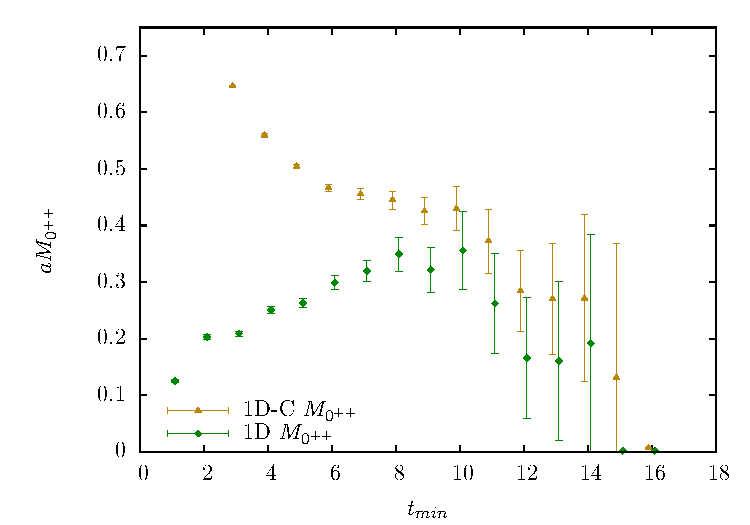
\includegraphics[width=2.5in]{./%ENSEMBLE%/plots/m0pp_zcen_cmp.pdf}\\
	\caption{Masses from non-linear fits from $t_{min}$ to the center of the correlator $N_t/2$.}
\end{figure}
\columnbreak
\begin{figure}[H]
\centering
    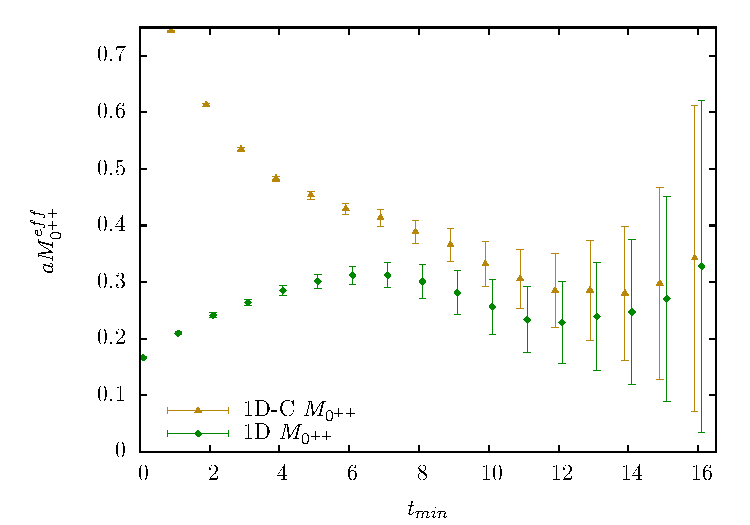
\includegraphics[width=2.5in]{./%ENSEMBLE%/plots/m0pp_zcen_eff.pdf}\\
	\caption{Kuti-style effective mass plots. }
\end{figure}
\end{multicols}

\begin{multicols}{2}
	\begin{figure}[H]
\centering
        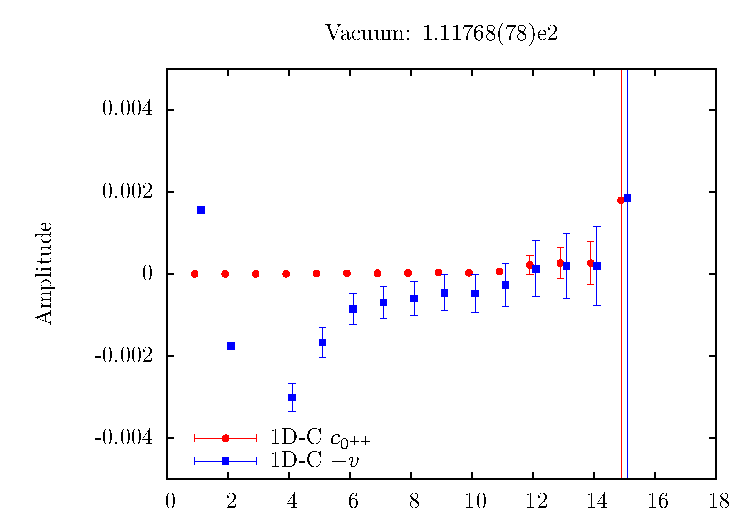
\includegraphics[width=2.5in]{./%ENSEMBLE%/plots/m0pp_zcen_amp.pdf}\\
	\caption{Amplitude and vacuum comparison (%NF%D-C) from non-linear fits from $t_{min}$ to the center of the correlator $N_t/2$.}
\end{figure}
\columnbreak
\begin{figure}[H]
\centering
    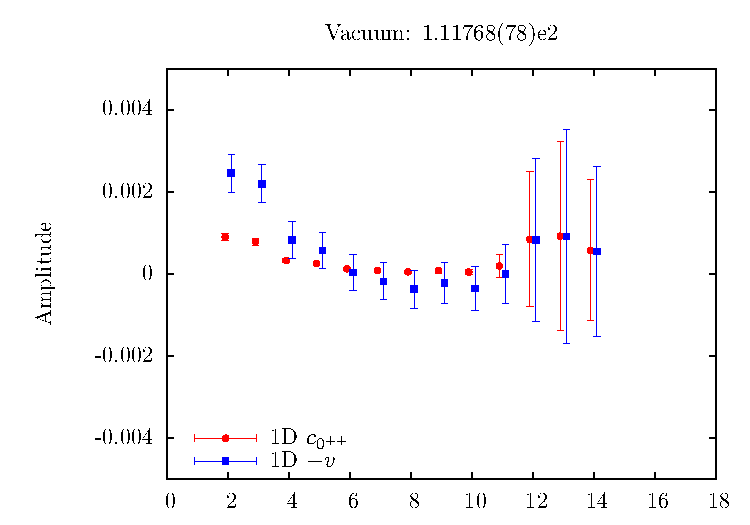
\includegraphics[width=2.5in]{./%ENSEMBLE%/plots/m0pp_zcen_amp_dc.pdf}\\
	\caption{Amplitude and vacuum comparison (%NF%D) from non-linear fits from $t_{min}$ to the center of the correlator $N_t/2$.}
\end{figure}
\end{multicols}

\begin{multicols}{2}
	\begin{figure}[H]
\centering
        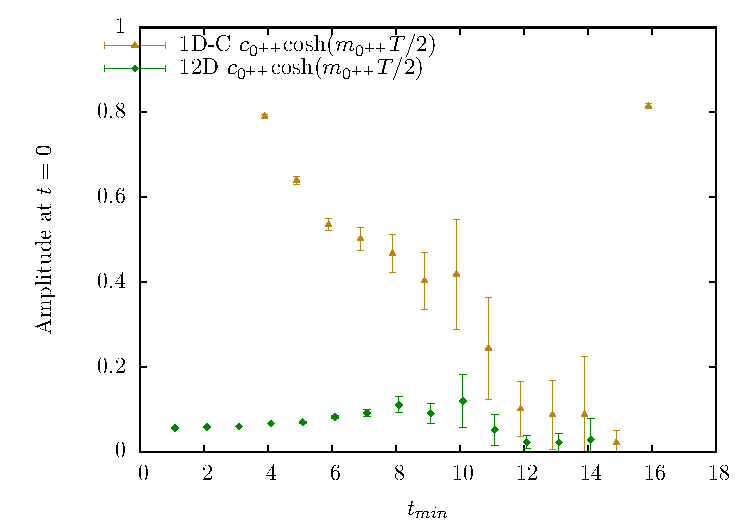
\includegraphics[width=2.5in]{./%ENSEMBLE%/plots/m0pp_zcen_amp_orig.pdf}\\
	\caption{Amplitude (propagated back to $t=0$) from non-linear fits from $t_{min}$ to the center of the correlator $N_t/2$.}
\end{figure}
\columnbreak
\begin{figure}[H]
\centering
        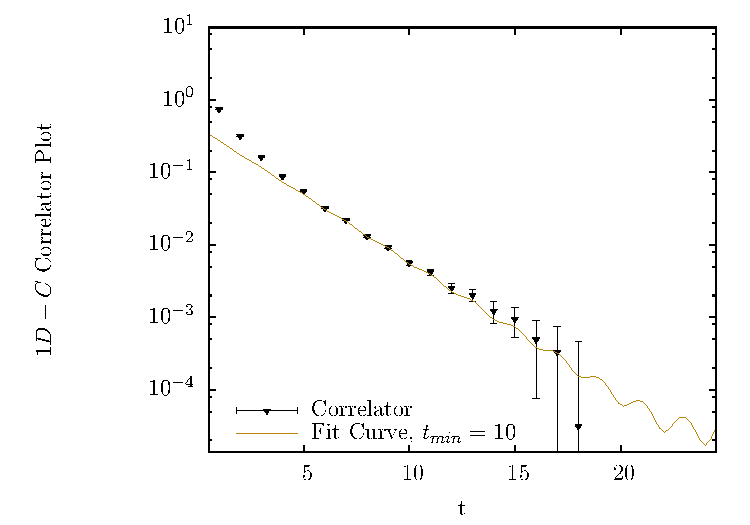
\includegraphics[width=2.5in]{./%ENSEMBLE%/plots/m0pp_zcen_fitlines.pdf}\\
        \caption{A sample fit of the data to a fit form. We look at %CORRNAME% using results from $t_{min} = %CORRTMIN%$.}
\end{figure}

\end{multicols}

